%!TEX root = ../thesis.tex
\chapter{Software Architecture}
\label{chap:architecture}

In this chapter, the composition of the system is described with more detail. One of the challenges when developing SAJaS was deciding how to implement assynchronous JADE-based features in a tick-based environment. This is described in Section \ref{sec:agentexecution}. Following it is the definition of the architecture of the system in the form of conceptual diagrams. Closing this chapter is a discussion on the extension perspectives of the system.

\section{Agent Execution in SAJaS}
\label{sec:agentexecution}

% Agent execution in JADE and Repast
As described in Section \ref{sec:jade-repast}, JADE execution can be concurrent and parallel, since JADE supports distributed and multi-threaded agent systems. Execution in Repast, on the other hand, is not concurrent. Repast uses a time-share type of execution, granting each agent the right to perform its tasks until they finish them, in sequence, but in no particular order.

% Agent execution in the API
\subsection{Asynch-like execution in Repast}
Except when executed during their setup or takedown, agents' actions in JADE are encapsulated in Behaviours. In JADE, multiple agents can be executing their behaviours simultaneously. In Repast, however, all scheduled objects run consecutively with variable execution sequence. This schedule is one of the components in SAJaS that is specific to its Repast interface. How behaviours are scheduled can be defined by the programmer.

Even though a local application can take advantage of direct method invocation, when the simulation platform is single-threaded - as Repast is - there is a risk of the simulation stagnating if, for instance, two agents engage in a very long ``conversation''.

Figure \ref{fig:direct_method_execution} represents a scenario where two agents engage in a conversation that involves multiple multiple replies from both sides. With direct method invocation, the response is instantaneous but other agents don't get any time to execute in-between.

In Figure \ref{fig:assynch_execution} on the other and, each agent is allowed to execute one task - send one message, in this case. Messages stay waiting until the agent reads and processes it. This way, Agent C didn't have to wait  for the other two to finish.

\begin{figure}[ht]
	\centering
    \begin{subfigure}[b]{\linewidth}
		\centering
		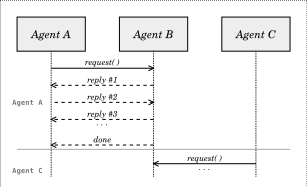
\includegraphics[width=.7\linewidth]{figures/executionProblem.pdf}
		\caption{
			With direct method invocation
		}
		\label{fig:direct_method_execution}
    \end{subfigure} \\
    \begin{subfigure}[b]{\linewidth}
		\centering
		\includegraphics[width=.7\linewidth]{figures/executionProblem2.pdf}
		\caption{
			Asynchronously 
		}
		\label{fig:assynch_execution}
    \end{subfigure}
    \caption[Time sharing example]{Smaller time ``allowances'' favour fair time sharing}
    \label{fig:execution_problems}
\end{figure}

In \cite{mengistu2008scalability}, authors concluded that increasing the granularity of the system, it is possible to improve its overall performance, even if individual tasks are delayed. The granularity of an agent task is explained as the communication-to-computation, or ``a measure of the amount of computation an agent executes before entering the communication phase of one simulation time step''.

In SAJaS, as in JADE, agent interaction occurs using the messaging service. Therefore, asynchronous execution is appropriate for the kind of applications developed for JADE and SAJaS. Simulations in Repast, though, usually depend on the synchrony of the environment. The use of ACLMessages, which wait in the message queue until processed, allows to maintain a synchronous execution, while simulating an asynchronous one.

To better demonstrate the differences between agent execution in both frameworks, Figure \ref{fig:execution_example} represents a scenario where two agents send a message to a third one who then replies. In SAJaS (Fig. \ref{fig:com-example-repast}), messages are delivered to agent C's message queue, and processed only in C's turn. In JADE (Fig. \ref{fig:com-example-jade}), messages can arrive concurrently. Their arrival triggers an event and they are processed right away in the receiving agent's thread. In this case, agent C handles the messages as they arrive and issues the respective replies.

\begin{figure}
	\centering
    \begin{subfigure}[b]{\linewidth}
		\centering
		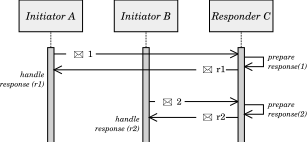
\includegraphics[width=0.7\linewidth]{figures/tickExample2.pdf}
		\caption{
			In JADE, running in parallel
		}
		\label{fig:com-example-jade}
    \end{subfigure}
    \vspace{1cm}
    \begin{subfigure}[b]{\linewidth}
		\centering
		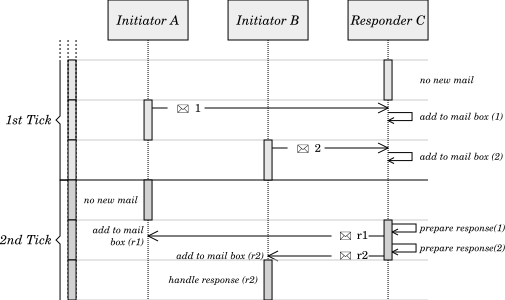
\includegraphics[width=0.9\linewidth]{figures/tickExample.pdf}
		\caption{
			In \apiname{}.
		}
		\label{fig:com-example-repast}
    \end{subfigure}
    \caption{Communication and agent interaction}
    \label{fig:execution_example}
\end{figure}


While the diagram above represents the agents as scheduled objects, their behaviours are the ones actually being scheduled and one agent typically initiates multiple behaviours. It is worth noting that the order by which Repast executes each scheduled behaviour is not predictable. To remove the influence that a fixed execution order can have in the outcome of a simulation, the schedule is randomized every tick. As a result, it is not guaranteed that all the behaviours of a single agent are executed consecutively. This is the expected execution when working with Repast as well as with JADE (given its multi-threaded nature) and it is up to the programmer to ensure that the application does not rely on the order of execution.

\subsection{Messaging issues}
\label{sec:mess_issues}
An issue arose while testing multiple concurrent sessions of agent interaction, as in the case of the second experiment in Chapter \ref{chap:validation}. The initial implementation of the interaction protocols in SAJaS would receive up to one message from the agent's mail queue in each tick. If the agent would receive N CFPs, then it would take at least N ticks to process them all. While this didn't raise any problem with a single session scenario, with multiple sessions, contract net initiators would start to initiate protocols faster than the responders would terminate them. For this reason, SAJaS was changed so that when possible, all matching ACLMessages should be processed in a single tick.

\section{SAJaS Architecture}

From the point of view of the MAS programmer, working with this API feels the same as working with JADE, although limited to the presently available features. However, SAJaS has a much simpler internal architecture, which attempts to implement only the fundamental components needed for everything else to work. The most evident feature that was not ported from JADE was the network layer that enables the creation of distributed MAS.

Section \ref{sec:arch_conceptual} provides a broad overview of the whole system, followed by a deeper analysis of the implementation of the behaviours and protocols in Section \ref{sec:arch_behaviours}. Section \ref{sec:arch_interface} explains SAJaS' interfacing points, i.e. the way the programmer can effectively use the API.

\subsection{Conceptual Model}
\label{sec:arch_conceptual}
The diagram in Figure \ref{fig:arch} represents the internal architecture of SAJaS. The module captioned ``My Implementation'' represents an hypothetical implementation of a MABS that uses SAJaS. The ``Repast Simphony'' package's purpose is to represent the dependence of one of SAJaS classes to Repast libraries.

Within the API, three different categories of classes are represented.

\begin{enumerate}
	\item First, inside the ``Repast'' package are the classes that are specific to the Repast implementation of SAJaS. Repast contains an interface called ``ContextBuilder'' which contains the build method, the first one called when the simulation is initiated.
\end{enumerate}


Second, classes whose border is dotted are internal classes that are not meant to be used by programmers; some are not present in JADE and therefore their use cannot be ported by the conversion tool. Finally, the rest rest of the classes are the ones that programmers are expected to use and are directly supported by JADE and by the code conversion tool.

\begin{figure}[h]
	\centering
	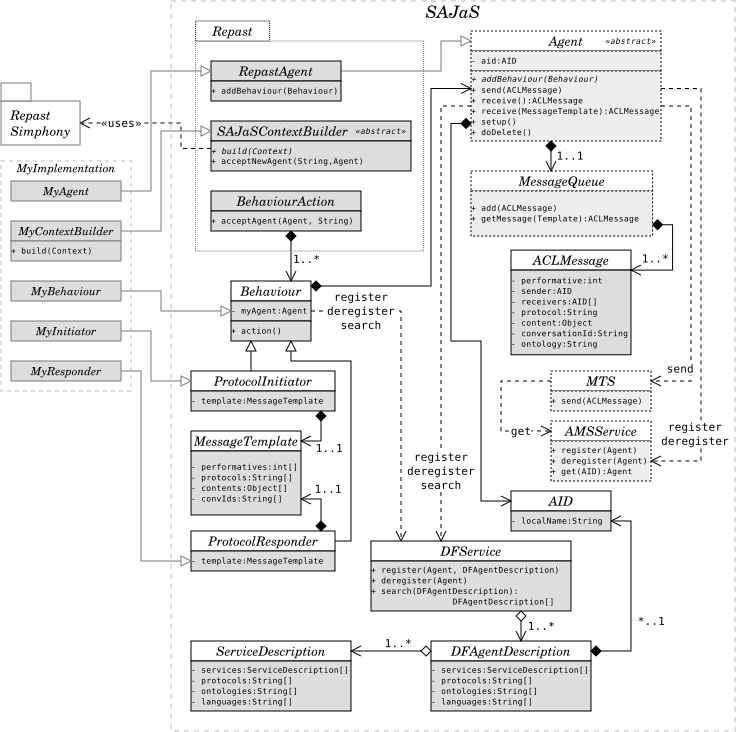
\includegraphics[width=\linewidth]{figures/sajas_arch.pdf}
	\caption[\apiname{}'s architecture]{Architecture of \apiname{}. The classes with doted border are internal.}
	\label{fig:arch}
\end{figure}

While tasks can be performed during agent setup and takedown, in runtime they are typically executed inside Behaviours. In the diagram, the Behaviour, the Protocol Initiator and the Protocol Responder are actually representations of a family of classes. For simplicity of this diagram, their complete representation is isolated in Figure \ref{fig:arch_proto}.

An agent in \apiname{} contains a MessageQueue which holds its queue of ACLMessages that are yet to be processed. The behaviours access to the agent who owns them and can call \texttt{receive()} on it to obtain the next message that matches the a template.

The DFService, as described before, provides the yellow page service. Agents can register or deregister themselves from the DF and perform searches. The DF contains a set of DFAgentDescriptions that describe agents and the services they perform. To quickly fetch agents when a search query arrives, the DF contains a mapping of the agents that are registered with each service, protocol, ontology and language. That means that, internally, the Directory Facilitator actually contains multiple sub-directories.

Agent interaction is always established through the use of ACLMessages. At no point to agent have access to other agents. Agents use an AID to identify themselves and other Agents. Besides the Agent itself, only the AMSService knows the address corresponding to an AID.

Behaviours that implement interaction protocols contain a MessageTemplate. This template is not fixed, but changes depending on the state of the protocol. The template is used to retrieve one message at a time from the agent's MessageQueue. One template can match multiple ACLMessages in the queue, but it always returns one single message.

\subsection{Behaviours and Protocols}
\label{sec:arch_behaviours}
Figure \ref{fig:arch_proto} represents the Behaviours with more detailed, as implemented by SAJaS. The Behaviour superclass contains methods that re triggered by certain events.

\begin{enumerate}
	\item \texttt{action} is called once per tick
	\item \texttt{onStart} is called immediately before the first call to \texttt{action}
	\item \texttt{onEnd} is called right after the behaviour ended;
	\item \texttt{done} is called every tick to determine if the behaviour has ended and if true is returned, it triggers \texttt{onEnd}.
\end{enumerate}

The methods \texttt{action} and \texttt{done} are abstract in Behaviour, so  other behaviours have to implement it. Methods \texttt{onStart} and \texttt{onEnd}, though, are implemented but do nothing in Behaviour.

The five ``responder'' and ``initiator'' classes implement the two protocols currently available in SAJaS. The FSMBehaviour, which they extend, contains a dynamic list of states and transitions. These can be registered and unregistered at runtime, typically before initiating the behaviour or in its setup. Each state is itself a behaviour.

Each protocol can be represented as a different state machine. For instance, in a Contract Net, the initiator's state starts as ``sending CFP'', then ``waiting for replies'', ``waiting for result notifications'' and finally ``finished''. Protocols in SAJaS were initially implemented using Java \texttt{enum}s. An \texttt{enum}\footnote{http://docs.oracle.com/javase/tutorial/java/javaOO/enum.html} is an immutable variable type that can only take a predefined set of constant values.

Even though it is important to preserve JADE-like execution, simplifying non-essential internal features that are invisible to the programmer provides increased performance. Tests were performed to decide whether these behaviours should use \texttt{enum}s or the dynamic FSM. Three possible solutions were tested:

\begin{enumerate}
	\item \textbf{First}, a JADE-like approach where each state is a Behaviour in a dynamic FSM;
	\item \textbf{Second}, an hybrid approach, using a single state in a dynamic FSM, where that state is an \texttt{enum} containing the actual FSM; this approach is more faithful to JADE's than using olely \texttt{enum}s;
	\item \textbf{Third}, a pure \texttt{enum}-based approach.
\end{enumerate}

Using the contract net scenario describe further ahead in Chapter \ref{chap:validation}, the performance of these approaches was compared. A pure \texttt{enum}-based FSM was shown to be significantly faster than a dynamic FSM. For this reason, the \texttt{enum}-based approach was kept and overrides the dynamic FSM from the superclass. The FSMBehaviour was also kept to allow the creation of custom behaviours by programmers using SAJaS.

\begin{figure}
	\centering
	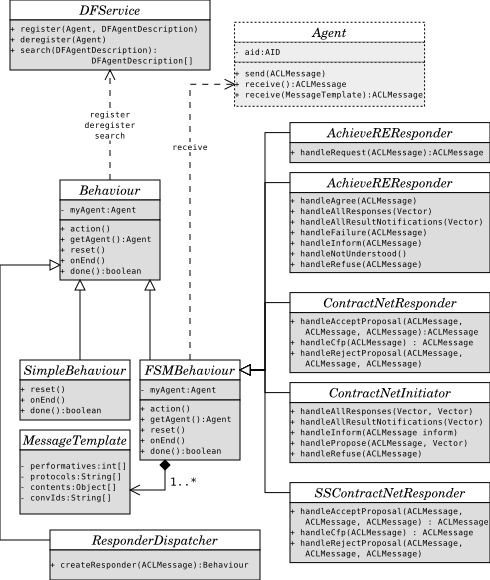
\includegraphics[width=0.7\linewidth]{figures/sajas_arch_proto.pdf}
	\caption[Behaviours and protocols in SAJaS]
	{Details of the Behaviours and Protocols in SAJaS}
	\label{fig:arch_proto}
\end{figure}

\subsection{Using SAJaS}
\label{sec:arch_interface}
To use SAJaS, it is important to understand how it should be interfaced. As explained earlier, the classes that are represented with a dotted border in Figure \ref{fig:arch} are internal and not supposed to be used by programmers because there is no JADE support for them. For programmers with experience in JADE, using SAJaS is very straightforward, although not all features all present.

Creating agents in SAJaS should be done using the appropriate implementation aimed at the simulation framework -- RepastAgent, in this case. The Agent class in SAJaS is abstract and implementing it directly would require the reimplementation of abstract methods by each agent. Specifically, the \texttt{addBehaviour} method schedules a Behaviour and this scheduler is part of the simulation tool.

Creating Behaviours is also done using one of the already implemented subclasses. Each protocol behaviour, for instance, contains a series of message handlers that should be implemented when needed.

The messaging service is accessed through the \texttt{receive} and \texttt{send} methods in the Agent class. The DF Service is also accessible directly through the DFService class.

For MABS based on SAJaS and Repast, a program launcher must implement the Repast interface \texttt{ContextBuilder}. The \texttt{SAJaSContextBUilder} class implements it in order to provide an extra abstraction layer from repast. To create a Repast launcher, the programmer should extend \texttt{SAJaSContextBUilder} and implement the \texttt{setup} method. The ContextBuilder does not exist in JADE and therefore, conversion doesn't yet create a runnable JADE application. However, all that needs to be done is to call the \texttt{setup} method from within the JADE main class.


\section{Extension Perspectives}

SAJaS was developed keeping in mind the possibility to create extensions to it's features in the future. While this thesis was initially focused on providing Repast with support for FIPA standards for agent interaction (and all the infrastructure that supports it), the API evolved to incorporate many more JADE-based features. It is purposely generic and to allow support for other simulation development tools to be added will few changes to the API itself. To support another framework, a scheduling mechanism should be crated that is appropriate for that framework. That scheduler should run call the BehaviourAction one per ``tick''.

The plugin is closely related to SAJaS, so updates to SAJaS will demand changes to the plugin as well. To facilitate the update of the plugin, it relies on a dictionary file that contains a mapping of the classes between SAJaS and JADE. The dictionary also supports some annotations that allow more that just a direct translation between two classes.




%Figure \ref{fig:arch} illustrates the details of \apiname{}'s architecture. Most concepts represented in this diagram are present in JADE, namely the Agent, ACL Message, Behaviour, MTS and DF service.
%
%An agent in \apiname{} contains a MessageQueue and a set of Behaviours. These have access to the agent who owns them and to its MessageQueue. A behaviour that implements an interaction protocol makes use of MessageTemplates. These are used to retrieve relevant messages in each step of the protocol. The MessageTemplates are updated while the protocols go through their different states.
%
%The DFService, as described before, provides the yellow page service. Agents can register or deregister themselves in the DF as well as perform searches. While tasks can be performed during agent setup, in runtime they are typically executed inside Behaviours.
%
%To follow JADE-like communication, ACL Messages carry agent identifiers (AID) for senders and receivers. These AIDs are returned by the DF as search results and are resolved to an agent by the MTS when sending a message. In \apiname{} the MTS keeps a mapping of AIDs to agents for easier access.
%
%The ``plug-in points'' of the API are the Agent, the Behaviour and their derived classes. The API also supports direct access to the DFService. In Figure \ref{fig:arch} all protocol definitions are implied by the generic sub-classes ``ProtocolInitiator'' and ``ProtocolResponder''. 
%
